\documentclass[../rgr1.tex]{subfiles}
\usetikzlibrary{shapes.geometric,angles,quotes}

\begin{document}

\Problem{
	Знайти найбільше і найменше значення елементів геометричних фігур
}
	Через точку $A (2; 1/4)$ проводяться прямі, що перетинають
	додатні півосі в точках $B$ і $C$. Знайти рівняння тієї
	прямої, для якої відрізок $BC$ має найменшу довжину.

\Solution

\begin{wrapfigure}{l}{5cm}
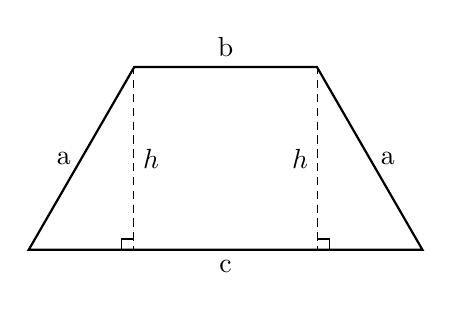
\begin{tikzpicture}[my angle/.style={font=\scriptsize, draw, angle eccentricity=1.75, angle radius=3mm}]
  \node (a) [trapezium, trapezium angle=60, minimum width=50mm, draw, thick, label=above:b, label=below:c, label=right:a, label=left:a] {};
  \draw [densely dashed] (a.north west) coordinate (a nw) -- (a nw |- a.south) node [midway,right] {$h$} coordinate (a1) (a.north east) coordinate (a ne) -- (a ne |- a.south) node [midway,left] {$h$} coordinate (a2);
  \draw (a nw |- a.south) ++(0,1.5mm) -| ++(-1.5mm,-1.5mm) (a ne |- a.south) ++(0,1.5mm) -| ++(1.5mm,-1.5mm);
  \coordinate (a blc) at (a.bottom left corner);
  \coordinate (a brc) at (a.bottom right corner);
  % \pic [my angle, "$\alpha$"] {angle=a1--a blc--a nw};
  % \pic [my angle, "$\alpha$"] {angle=a ne--a brc--a1};
  % \pic [my angle, "$\beta$"] {angle=a blc--a nw--a1};
  % \pic [my angle, "$\beta$"] {angle=a2--a ne--a brc};
\end{tikzpicture}
\end{wrapfigure}

Позначимо бічну сторону трапеції як $a$, верхню основу як $b$, нижню основу як $c$, висоту як $h$, площу як $S$, а кут між бічною стороною та нижньою основою як $\alpha$. Оскільки трапеція є рівнобедреною, то $a=c$.

Запишемо формулу для площі трапеції:
$$S=\frac{(b+c)h}{2}$$
Оскільки $a=c$, то $b=a+2h\tan\frac{\alpha}{2}$. Підставимо це вираз для $S$:
$$S=\frac{(a+c)(h+a\tan\frac{\alpha}{2})}{2}$$
$$S=\frac{(a+a)(h+a\tan\frac{\alpha}{2})}{2}$$
$$S=ah+a^2\tan\frac{\alpha}{2}+ \frac{h^2\tan\frac{\alpha}{2}}{2}$$
Отримали квадратичну функцію відносно змінної $a$, яку можна мінімізувати за допомогою пошуку вершини параболи.

Знайдемо похідну від $S$ за $a$:
$$\frac{dS}{da}=h+2a\tan\frac{\alpha}{2}$$
Прирівнюємо до нуля:
$$h+2a\tan\frac{\alpha}{2}=0$$
$$a=-\frac{h}{2\tan\frac{\alpha}{2}}$$
Це єдине критичне значення $a$ для мінімуму функції $S$.

Оскільки ми шукаємо довжину бічної сторони, то $a=c=-\frac{h}{2\tan\frac{\alpha}{2}}$.

Перевіримо, що це дійсно мінімум:
$$\frac{d^2S}{da^2}=2\tan\frac{\alpha}{2}>0$$
Отже, знайдене значення $a$ є точкою мінімуму функції $S$.

Отже, довжина бічної сторони трапеції, що має найменший периметр, дорівнює $-\frac{h}{2\tan\frac{\alpha}{2}}$.
<++>

\Answer{<++>}
\end{document}
